%!TEX root = ../main.tex

\chapter{Tipi di costellazioni satellitari}
\label{chp:intro}

Una costellazione di Internet via satellite è una costellazione di satelliti artificiali che forniscono servizi di Internet. In particolare, il termine si riferisce a una nuova generazione di costellazioni molto grandi (a volte indicate come megacostellazioni) che orbitano nell'orbita terrestre bassa (LEO) per fornire servizi Internet a bassa latenza e ad alta larghezza di banda (banda larga) \cite{jose_del_rosario_nsr_2018}.
% Nel 2020, il 63\% delle famiglie che vivono in zone rurali del mondo non ha accesso a Internet a causa dei requisiti infrastrutturali dei cavi sotterranei e delle torri di rete. Le costellazioni Internet via satellite offrono una soluzione a basso costo per espandere la copertura \cite{makena_young_low_2022}.
A novembre 2022, poco più del 63\% degli 8 miliardi di persone nel mondo utilizza Inetrnet, lasciando circa 3 miliardi di persone (e potenziali clienti) non connnessi.
Per colmare questo divario digitale, governi e aziende commerciali private stanno investendo in iniziative per costruire Internet a banda larga basata sullo spazio.
Se avranno successo, questi sforzi hanno il potenziale per connettere rapidamente le persone in tutto il mondo e cambiare l'ambiente spaziale stesso.
Diversi paesi stanno lanciando iniziative nazionali per stabilire costellazioni di satelliti in orbita terrestre bassa (\ac{LEO}) e catturare ampie porzioni di un mercato in crescita, liberando ampie risorse private o statali per farlo.

La competizione per fornire servizi a banda larga dai satelliti non è una novità.
Gli anni '90 hanno visto un simile boom commerciale di Internet a banda larga che ha prodotto scarso successo.
Aziende come Teledesic, Celestri, Globalstar e Iridium hanno tutte proposto grandi costellazioni di comunicazioni satellitari (SATCOM) in \ac{LEO}, ma quasi tutte sono finite in bancarotta all'inizio degli anni 2000.

Oggi la barriera all'ingresso in orbita è notevolmente diminuita poichè la tecnologia, i materiali e le capacità di lancio sono diventati più economici e più ampiamente disponibili.
La concorrenza internazionale per costruire, langiare e gestire un sistema a basso costo e bassa latenza che si estenda in tutto il mondo è feroce, poichè la domanda di servizi internet veloci e affidabili continua a crescere.

A partire dal 2022, solo un operatore, Starlink, fornisce un servizio basato su \ac{LEO} sul mercato libero.
Si stima che il mercato globale SATCOM crescerà fino a 40 miliardi di dollari entro il 2030, in gran parte guidato da iniziative basate su \ac{LEO}.

L'istituzione di una costellazione \ac{LEO}, comporta un investimento iniziale sostanziale, un know-how tecnico specializzato e la capacità di orientarsi in un panorama normativo complesso.
Con l'intensificarsi della concorrenza internazionale nelle comunicazioni \ac{LEO}, è fondamentale che il governo degli stati uniti crei un ambiente normativo abilitante (ma robusto) affinchè le imprese con sede negli Stati Uniti possano prosperare in patria e all'estero.

Il più grande concorrente degli Stati Uniti nella corsa alla connettività globale tramite banda larga satellitare è la Cina.
La Cina ha proposto una costellazione di 13000 satelliti in \ac{LEO} per soddisfare le esigenze residenziali e aziendali nel mercato cinese, nonchè nei mercati Internet sottosviluppati in tutto il mondo \cite{makena_young_low_2022}.

\section{Vantaggi della Low Earth Orbit}

I satelliti sono tipicamente lanciati in una di tre orbite: Low Earth Orbit (\ac{LEO}) dai 160 ai 2'000 km, Medium Earth Orbit (\ac{MEO}) dai 2000 ai 35786 km, o Geosynchronous Orbit (GEO) a 42164 km.
Ciascuna delle tre orbite ha i suoi vantaggi.
Per esempio, una costellazione in GEO può avere copertura globale con solo tre satelliti per la sua distanza dalla superficie terrestre.
La GEO è popolare per le comunicazioni per questo motivo.
Però, dato che i satelliti sono così distanti dalla Terra la latenza è molto alta.

\begin{figure}[htbp]
  \centering
  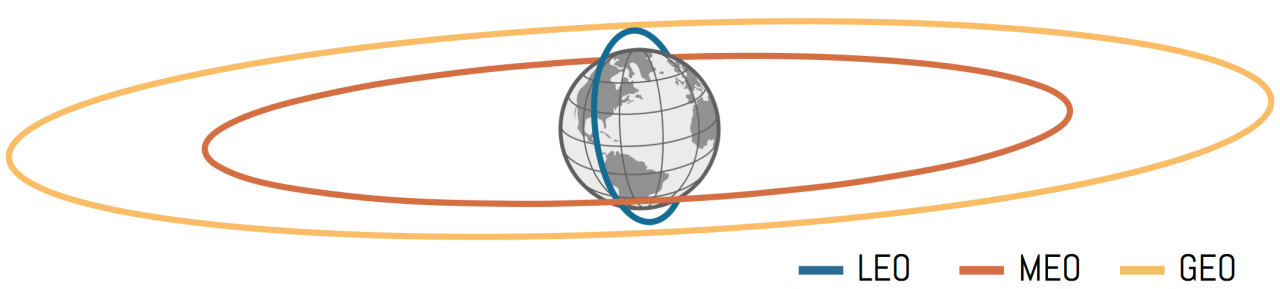
\includegraphics[width=0.9\linewidth]{./res/img/leo_orbit.png}
  \caption{Orbite terrestri di popolare utilizzo \cite{thomas_g_roberts_popular_2022}}
  \label{fig:leo-orbit}
\end{figure}

Le nuove generazioni di internet via satellite stanno collocando i satelliti in \ac{LEO} invece della tradizionale \ac{GEO} per una serie di motivi.
Infatti i satelliti lanciati in \ac{LEO} sono tipicamente più piccoli e più leggeri di quelli in \ac{GEO}, quindi serve meno carburante per mandarli in orbita e in generale sono ridotti i costi di lancio.
Inoltre, dato che i satelliti sono più vicini i terminali utente possono rilevare più satelliti allo stesso tempo e conettersi quindi al satellite più conveniente.

Le comunicazioni dalla \ac{LEO} hanno anche una latenza inferiore rispetto ai satelliti in \ac{GEO} perchè sono molto più vicini alla superficie terrestre.
Gli operatori satellitari \ac{LEO} sostengono che una pagina web può essere aperta circa otto volte più velocemente quando si utilizzano i satelliti \ac{LEO} rispetto a quando si utilizza un sistema SATCOM tradizionale in \ac{GEO}, qualcosa che è diventato più importante per i consumatori che vogliono interagire online quasi in tempo reale.
Ciò significa che Internet satellitare deve essere in grado di supportare applicazioni ad alta velocità come streaming, videoconferenza e giochi in tempo reale \cite{makena_young_low_2022}.

% https://en.wikipedia.org/wiki/SpaceX#Starlink_2
\section{Starlink}

Starlink è una costellazione internet via satellite operata da Starlink Services LLC, una consociata interamente controlla dalla società aerospaziale americana SpaceX, che fornisce copertura a oltre 100 paesi e territori.
Mira inoltre a firnire la banda larga mobile a livello mondiale.

SpaceX ha iniziato a lanciare i satelliti Starlink nel 2019.
A partire da settembre 2024, la costellazione è composta da oltre 7000 piccoli satelliti prodotti in serie in orbita terrestre bassa (\ac{LEO}) che comunicano con terminali utente sulla Terra \cite{jonathan_mcdowell_starlink_nodate}.
SpaceX prevede di schierare quasi 12000 satelliti, con una prossibile estensione successiva a 34400.
SpaceX ha annunciato di aver raggiunto più di 1 milione di abbonati nel dicembre 2022 e 4 milioni di abbonati nel settembre 2024 \cite{starlink_starlink_nodate}.

Nel maggio 2018, SpaceX ha stimato che il costo totale della progettazione, costruzione e dispiegamento della costellazione sarebbe stato di almeno 10 milardi di dollari \cite{michael_baylor_block_2018}.
Secondo quanto riferito, i ricavi di Starlink nel 2022 sono stati di 1.4 milardi di dollari, accompagnati da una perdita netta, con un piccolo profitto iniziato solo nel 2023.
Si prevede che i ricevi raggiungeranno i 6.6 milardi di dollari nel 2024 \cite{eric_berger_analyst_2024}.

Gli astronomi hanno espresso preoccupazione sull'effetto che la costellazione potrebbe avere sull'astronomia da terra e su come i satelliti contribuiranno a un ambiente orbitale già congestionato.
SpaceX ha tentato di mitigare i problemi di interferenza astronomica con misure per ridurre la luminosità dei satelliti durante il funzionamento.
I satelliti sono dotati di propulsori ad effetto Hall che consentono loro di alzare l'orbita, mantenere una posizione di stazionamento e uscire dall'orbita alla fine della loro vita.
Sono inoltre progettati per evitare collisioni in modo autonomo e senza intoppi sulla base dei dati di tracciamento collegati in uplink \cite{spacex_astronomy_2020}.